\documentclass[12pt,a4paper]{article}

% ─── Page Layout ───────────────────────────────────────────────────────────────
\usepackage[a4paper, margin=0.8in, headheight=14pt]{geometry}

% ─── Fonts (XeLaTeX) ───────────────────────────────────────────────────────────
\usepackage{fontspec}
\usepackage{unicode-math}
\setmainfont{TeX Gyre Pagella}
\setmonofont[Scale=0.88]{TeX Gyre Cursor}
\setmathfont{Latin Modern Math}

% ─── Packages ──────────────────────────────────────────────────────────────────
\usepackage{xcolor}
\usepackage{colortbl}
\usepackage{titlesec}
\usepackage{enumitem}
\usepackage{tabularx}
\usepackage{booktabs}
\usepackage{array}
\usepackage{amsmath}
\usepackage{tikz}
\usetikzlibrary{shapes.geometric, arrows.meta, positioning, calc, fit, decorations.pathreplacing}
\usepackage{tcolorbox}
\tcbuselibrary{skins, breakable}
\usepackage{hyperref}
\usepackage{fancyhdr}
\usepackage{graphicx}
\usepackage{microtype}
\usepackage{caption}
\usepackage{setspace}
\usepackage{multirow}
\usepackage{tocloft}

% ─── Q&A helper ────────────────────────────────────────────────────────────────
\newcommand{\Q}[1]{\textbf{#1}\par\noindent\ignorespaces}

% ─── Colour Palette ────────────────────────────────────────────────────────────
\definecolor{myred}{RGB}{196,30,58}
\definecolor{mydark}{RGB}{30,30,50}
\definecolor{mygreen}{RGB}{14,120,80}
\definecolor{myteal}{RGB}{0,130,140}
\definecolor{myamber}{RGB}{180,100,0}
\definecolor{mypurple}{RGB}{100,30,160}
\definecolor{mygray}{RGB}{246,247,249}
\definecolor{mgframe}{RGB}{180,185,200}
\definecolor{watermark}{RGB}{145,150,170}
\definecolor{hdrred}{RGB}{250,232,235}
\definecolor{hdrgreen}{RGB}{220,244,233}
\definecolor{hdrteal}{RGB}{220,242,244}
\definecolor{hdramber}{RGB}{253,242,215}
\definecolor{hdrpurple}{RGB}{238,228,255}
\definecolor{hdrgray}{RGB}{238,240,245}
\definecolor{rowalt}{RGB}{250,251,253}

% ─── Section Formatting ────────────────────────────────────────────────────────
\titleformat{\section}
  {\large\bfseries\color{myred}}{\thesection.}{0.5em}{}
  [\vspace{1pt}{\color{myred}\rule{\linewidth}{0.8pt}}]
\titleformat{\subsection}
  {\normalsize\bfseries\color{myteal}}{\thesubsection}{0.5em}{}
\titlespacing*{\section}{0pt}{18pt}{7pt}
\titlespacing*{\subsection}{0pt}{11pt}{4pt}

% ─── Paragraph ─────────────────────────────────────────────────────────────────
\setlength{\parindent}{0pt}
\setlength{\parskip}{4pt}

% ─── TOC Styling ───────────────────────────────────────────────────────────────
\renewcommand{\cfttoctitlefont}{\large\bfseries\color{myred}}
\renewcommand{\cftaftertoctitle}{\par\noindent{\color{myred}\rule{\linewidth}{0.8pt}}}
\setlength{\cftbeforetoctitleskip}{0pt}
\setlength{\cftaftertoctitleskip}{6pt}
\renewcommand{\cftsecfont}{\normalsize\bfseries\color{mydark}}
\renewcommand{\cftsecpagefont}{\normalsize\bfseries\color{mydark}}
\renewcommand{\cftsecleader}{\cftdotfill{\cftdotsep}}
\setlength{\cftbeforesecskip}{7pt}
\renewcommand{\cftsubsecfont}{\small\color{mydark}}
\renewcommand{\cftsubsecpagefont}{\small\color{mydark}}
\setlength{\cftbeforesubsecskip}{3pt}
\setlength{\cftsubsecindent}{1.4em}

% ─── Table helpers ─────────────────────────────────────────────────────────────
\renewcommand{\arraystretch}{1.45}
\setlength{\tabcolsep}{6pt}
\newcolumntype{B}[1]{>{\small\bfseries\raggedright\arraybackslash}m{#1}}
\newcolumntype{Y}{>{\small\raggedright\arraybackslash}X}
\renewcommand{\tabularxcolumn}[1]{m{#1}}

% ─── Header / Footer ───────────────────────────────────────────────────────────
\pagestyle{fancy}
\fancyhf{}
\fancyhead[L]{\small\color{myred}\textbf{HS-HU601}\;\color{mydark}--- Economics for Engineers}
\fancyhead[R]{\small\color{myteal}\textbf{Module 2 Notes}}
\fancyfoot[C]{\small\color{mydark}\thepage}
\fancyfoot[R]{\small\color{watermark}\textit{\copyright\ Biraj}}
\renewcommand{\headrulewidth}{0.5pt}
\renewcommand{\footrulewidth}{0.3pt}

% ─── Hyperref ──────────────────────────────────────────────────────────────────
\hypersetup{
  colorlinks=true, linkcolor=myteal, urlcolor=myteal,
  pdfauthor={Biraj Sarkar},
  pdftitle={HS-HU601 --- Module 2 Notes}
}

% ─── tcolorbox styles ──────────────────────────────────────────────────────────
\tcbset{
  tikzbox/.style={
    colback=mygray, colframe=mgframe, boxrule=0.6pt, arc=4pt,
    left=8pt, right=8pt, top=6pt, bottom=6pt,
    colbacktitle=mgframe, coltitle=mydark,
    fonttitle=\small\bfseries
  },
  defbox/.style={
    colback=hdrgreen, colframe=mygreen, boxrule=0.8pt, arc=4pt,
    left=9pt, right=9pt, top=6pt, bottom=6pt,
    colbacktitle=mygreen, coltitle=white,
    fonttitle=\small\bfseries
  },
  formulabox/.style={
    colback=hdrteal, colframe=myteal, boxrule=0.8pt, arc=4pt,
    left=9pt, right=9pt, top=7pt, bottom=7pt,
    colbacktitle=myteal, coltitle=white,
    fonttitle=\small\bfseries
  },
  examplebox/.style={
    colback=hdramber, colframe=myamber, boxrule=0.8pt, arc=4pt,
    left=9pt, right=9pt, top=6pt, bottom=6pt,
    colbacktitle=myamber, coltitle=white,
    fonttitle=\small\bfseries
  },
  masonbox/.style={
    colback=hdrpurple, colframe=mypurple, boxrule=0.8pt, arc=4pt,
    left=9pt, right=9pt, top=6pt, bottom=6pt,
    colbacktitle=mypurple, coltitle=white,
    fonttitle=\small\bfseries
  },
  exambox/.style={
    colback=hdrpurple, colframe=mypurple, boxrule=1pt, arc=5pt,
    left=10pt, right=10pt, top=8pt, bottom=8pt,
    colbacktitle=mypurple, coltitle=white,
    fonttitle=\bfseries,
    breakable
  }
}
% Make all boxes breakable across pages
\tcbset{breakable}

% ─── TikZ styles ───────────────────────────────────────────────────────────────
\tikzset{
  block/.style={rectangle, draw=myteal, fill=hdrteal,
    text width=2.4cm, align=center, minimum height=0.95cm,
    font=\small, rounded corners=3pt, line width=0.7pt},
  redblock/.style={rectangle, draw=myred, fill=hdrred,
    text width=2.4cm, align=center, minimum height=0.95cm,
    font=\small, rounded corners=3pt, line width=0.7pt},
  arrow/.style={-Stealth, thick, color=mydark},
  redarrow/.style={-Stealth, thick, color=myred},
  line/.style={thick, color=mydark}
}

% ═══════════════════════════════════════════════════════════════════════════════
\begin{document}
% ═══════════════════════════════════════════════════════════════════════════════

\begin{center}
  {\LARGE\bfseries\color{myred} HS-HU601 --- Economics for Engineers}\\[5pt]
  {\normalsize\color{mydark} Semester VI \quad$\bullet$\quad 3L:0T:0P \quad$\bullet$\quad 3 Credits}\\[3pt]
  {\normalsize\color{myteal}\textbf{Module 2 Exam Notes}}\\[3pt]
  {\small\color{mydark} CGEC \;$|$\; B.Tech ECE (2023--27) \;$|$\; \textit{Biraj Sarkar}}
\end{center}
\vspace{2pt}
\noindent{\color{myred}\rule{\linewidth}{1.5pt}}
\vspace{2pt}

\hypersetup{linkcolor=mydark}
\tableofcontents
\hypersetup{linkcolor=myteal}
\newpage

% ===============================================================================
\section{Cash Flow, Interest, and Equivalence}
% ===============================================================================

To evaluate engineering designs financially, we must track when money is spent and received.

\subsection{Cash Flow Diagrams}
A Cash Flow Diagram (CFD) is a graphical representation of cash flows plotted on a timeline.

\begin{tcolorbox}[defbox]
\textbf{Cash Inflow (Receipts):} Represented by vertical arrows pointing \textbf{upward} above the timeline (e.g., revenue, operating savings, salvage value).
\par\vspace{3pt}
\textbf{Cash Outflow (Disbursements):} Represented by vertical arrows pointing \textbf{downward} below the timeline (e.g., capital purchase, operating expenses, taxes).
\end{tcolorbox}

\begin{tcolorbox}[tikzbox, title={Typical Cash Flow Diagram for an Engineering Project}]
\centering
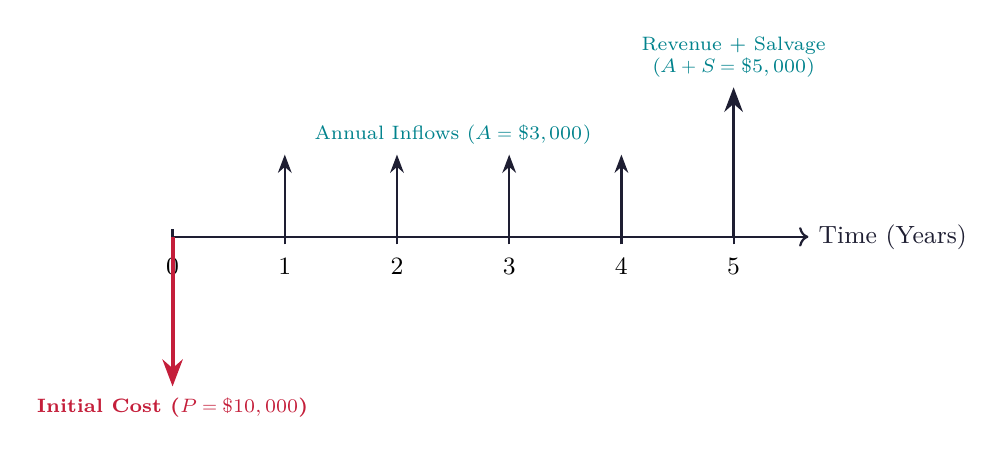
\begin{tikzpicture}[scale=0.95]
  % Timeline axis
  \draw[line, ->] (0,0) -- (8.5,0) node[right, font=\small] {Time (Years)};
  % Tick marks and labels
  \foreach \x/\lbl in {0/0, 1.5/1, 3.0/2, 4.5/3, 6.0/4, 7.5/5} {
    \draw[line] (\x, -0.1) -- (\x, 0.1);
    \node[below=4pt, font=\small] at (\x, 0) {\lbl};
  }
  
  % Outflow at t=0 (Initial Investment)
  \draw[redarrow, line width=1.5pt] (0,0) -- (0,-2.0) node[below, font=\scriptsize\bfseries\color{myred}] {Initial Cost ($P = \$10,000$)};
  
  % Annual Net Inflows at t=1..5
  \foreach \x/\t in {1.5/1, 3.0/2, 4.5/3, 6.0/4} {
    \draw[arrow] (\x,0) -- (\x, 1.1);
  }
  \node[above, font=\scriptsize\color{myteal}] at (3.75, 1.1) {Annual Inflows ($A = \$3,000$)};
  
  % Final Year inflow + Salvage Value at t=5
  \draw[arrow, line width=1.3pt] (7.5,0) -- (7.5, 2.0);
  \node[above, font=\scriptsize, align=center, color=myteal] at (7.5, 2.0) {Revenue + Salvage\\($A + S = \$5,000$)};
\end{tikzpicture}
\end{tcolorbox}

\subsection{Time Value of Money (TVM)}
The \textbf{Time Value of Money} states that a dollar received today is worth more than a dollar received in the future. This is due to three factors:
1.  \textbf{Opportunity Cost (Interest):} Capital can be invested to earn interest over time.
2.  \textbf{Inflation:} The purchasing power of money decreases over time.
3.  \textbf{Risk/Uncertainty:} Future receipts carry the risk of not being realized.

\subsection{Simple vs. Compound Interest}
\begin{itemize}[leftmargin=*, itemsep=6pt]
  \item \textbf{Simple Interest:} Calculated *only* on the original principal amount.
    \begin{equation}
      I = P \times i \times n
    \end{equation}
  \item \textbf{Compound Interest:} Interest is calculated on the principal *plus* any accumulated interest from previous periods.
    \begin{equation}
      F = P \times (1 + i)^n
    \end{equation}
\end{itemize}

\subsection{Nominal and Effective Interest Rates}
\begin{itemize}[leftmargin=*, itemsep=4pt]
  \item \textbf{Nominal Interest Rate ($r$):} The stated annual interest rate without considering compounding frequency within the year.
  \item \textbf{Effective Interest Rate ($i_a$):} The actual annual rate of interest paid or earned, accounting for compounding $m$ times per year.
\end{itemize}

\begin{tcolorbox}[formulabox, title={\textbf{Effective Interest Rate Formulas}}]
For a nominal rate $r$ compounded $m$ times per year:
\begin{equation}
  i_a = \left( 1 + \frac{r}{m} \right)^m - 1
\end{equation}
For continuous compounding ($m \to \infty$):
\begin{equation}
  i_a = e^r - 1
\end{equation}
\end{tcolorbox}

\subsection{Economic Equivalence}
Two cash flows (or series of cash flows) are \textbf{economically equivalent} at a given interest rate $i$ if they have the same financial value when discounted to the same point in time.

% ===============================================================================
\section{Time Value of Money Factors}
% ===============================================================================

To simplify calculations, standardized discount factors are used to convert cash flows between the Present ($P$), Future ($F$), and Uniform Series ($A$).


\subsection{TVM Factors Summary Table}
\par\noindent
{\renewcommand{\arraystretch}{1.9}%
\begin{tabularx}{\linewidth}{|B{3.2cm}|Y|Y|Y|}
\hline
\rowcolor{hdrteal}
\textbf{Find / Given} & \textbf{Factor Name} & \textbf{Standard Notation} & \textbf{Mathematical Formula} \\
\hline
Find $F$ given $P$ & Single Payment Compound Amount & $(F/P, i, n)$ & $(1+i)^n$ \\
\hline
\rowcolor{rowalt}
Find $P$ given $F$ & Single Payment Present Worth & $(P/F, i, n)$ & $(1+i)^{-n}$ \\
\hline
Find $F$ given $A$ & Uniform Series Compound Amount & $(F/A, i, n)$ & $\displaystyle\frac{(1+i)^n - 1}{i}$ \\[6pt]
\hline
\rowcolor{rowalt}
Find $A$ given $F$ & Sinking Fund & $(A/F, i, n)$ & $\displaystyle\frac{i}{(1+i)^n - 1}$ \\[6pt]
\hline
Find $A$ given $P$ & Capital Recovery & $(A/P, i, n)$ & $\displaystyle\frac{i(1+i)^n}{(1+i)^n - 1}$ \\[6pt]
\hline
\rowcolor{rowalt}
Find $P$ given $A$ & Uniform Series Present Worth & $(P/A, i, n)$ & $\displaystyle\frac{(1+i)^n - 1}{i(1+i)^n}$ \\[6pt]
\hline
\end{tabularx}}


\subsection{Debt Repayment (Loan Amortization)}
Amortization is the process of paying off debt through a series of equal periodic payments.
Each payment $A$ consists of two parts:
1.  \textbf{Interest Portion ($I_t$):} Computed on the outstanding loan balance at the beginning of period $t$.
2.  \textbf{Principal Portion ($P_t$):} The remaining part of the payment that reduces the outstanding loan balance.

\begin{tcolorbox}[formulabox, title={\textbf{Loan Amortization Equations}}]
For a loan principal $P$ at interest rate $i$ repaid over $n$ periods:
\begin{align}
  \text{Equal annual payment: } A &= P \times (A/P, i, n) = P \times \frac{i(1+i)^n}{(1+i)^n - 1} \\[6pt]
  \text{Interest in period } t: I_t &= B_{t-1} \times i \quad \text{($B_{t-1}$ is outstanding balance)} \\[4pt]
  \text{Principal reduction in } t: P_t &= A - I_t \\[4pt]
  \text{Remaining balance after } t: B_t &= B_{t-1} - P_t
\end{align}
\end{tcolorbox}

% ===============================================================================
\section{Cash Flow and Rate of Return Analysis}
% ===============================================================================

Engineers use standard analysis methods to determine if a project is financially viable.

\subsection{Present Worth, Future Worth, and Annual Worth Analysis}
\begin{itemize}[leftmargin=*, itemsep=6pt]
  \item \textbf{Present Worth (PW) Analysis:} All cash inflows and outflows are discounted to the present ($t=0$) at the Minimum Attractive Rate of Return (MARR).
    \begin{equation}
      PW(i) = \sum_{t=0}^{n} CF_t \times (1 + i)^{-t}
    \end{equation}
    \textit{Decision Rule:} Accept the project if $PW(MARR) \ge 0$.
  \item \textbf{Future Worth (FW) Analysis:} Cash flows are compounded to a future point ($t=n$). Useful for determining net accumulation at the end of project life.
  \item \textbf{Annual Worth (AW) Analysis:} Cash flows are converted into an equivalent uniform series over the project life.
    \begin{equation}
      AW(i) = PW(i) \times (A/P, i, n)
    \end{equation}
    \textit{Decision Rule:} Accept the project if $AW(MARR) \ge 0$.
\end{itemize}

\subsection{Internal Rate of Return (IRR) Analysis}
The \textbf{Internal Rate of Return (IRR)} is the interest rate at which the Present Worth of all cash flows equals zero.

\begin{tcolorbox}[formulabox, title={\textbf{IRR Equation}}]
\begin{equation}
  PW(IRR) = \sum_{t=0}^{n} \frac{CF_t}{(1 + IRR)^t} = 0
\end{equation}
*Decision Rule:* Accept the project if $IRR \ge MARR$.
\par\vspace{3pt}
\textbf{Linear Interpolation formula:} If trial rates $i_1$ (giving $PW_1 > 0$) and $i_2$ (giving $PW_2 < 0$) are close:
\begin{equation}
  IRR \approx i_1 + \left( \frac{PW_1}{PW_1 - PW_2} \right) \times (i_2 - i_1)
\end{equation}
\end{tcolorbox}

\subsection{Benefit-Cost Ratio (BCR) Analysis}
Often used in public sector projects to assess whether the societal benefits justify the public expenditure.

\begin{tcolorbox}[formulabox, title={\textbf{Benefit-Cost Ratio Formula}}]
\begin{equation}
  BCR = \frac{PV(\text{Benefits})}{PV(\text{Costs})} = \frac{PW(\text{Cash Inflows})}{PW(\text{Cash Outflows})}
\end{equation}
*Decision Rule:* Accept the project if $BCR \ge 1.0$.
\end{tcolorbox}

\subsection{Sensitivity and Breakeven Analysis}
\begin{itemize}[leftmargin=*, itemsep=6pt]
  \item \textbf{Sensitivity Analysis:} Determines how financial metrics (like PW or IRR) change when key parameters (like initial cost, useful life, or annual revenue) deviate from their estimated values.
  \item \textbf{Breakeven Analysis:} Determines the value of a parameter (e.g., production capacity, price, number of years) at which two alternatives become economically equivalent. At the breakeven point:
    \begin{equation}
      PW_A(i) = PW_B(i) \quad \text{or} \quad AW_A(i) = AW_B(i)
    \end{equation}
\end{itemize}

% ===============================================================================
\section{Worked Examples}
% ===============================================================================

\begin{tcolorbox}[examplebox, title={Example 1: Nominal vs. Effective Interest}]
\textbf{Problem:} An engineering company deposits $\$10,000$ in a bank account that pays a nominal interest rate of $12\%$ per year. Calculate the effective annual interest rate and the total balance after $5$ years under:
\begin{enumerate}[label=\alph*., leftmargin=*, itemsep=2pt, topsep=2pt]
  \item Quarterly compounding ($m = 4$).
  \item Continuous compounding.
\end{enumerate}
\textbf{Solution:}\\[4pt]
\textbf{(a) Quarterly Compounding ($m = 4$):}
\begin{align*}
  i_a &= \left( 1 + \frac{r}{m} \right)^m - 1 = \left( 1 + \frac{0.12}{4} \right)^4 - 1 = (1.03)^4 - 1 \\
  i_a &\approx 1.1255 - 1 = 12.55\%
\end{align*}
Future Balance after $5$ years ($n = 5 \times 4 = 20$ quarters, interest rate per quarter $= 3\%$):
\begin{align*}
  F &= P(1 + i)^{n_{quarters}} = 10,000 \times (1.03)^{20} \\
  F &\approx 10,000 \times 1.8061 = \$18,061
\end{align*}

\textbf{(b) Continuous Compounding:}
\begin{align*}
  i_a &= e^r - 1 = e^{0.12} - 1 \approx 1.1275 - 1 = 12.75\%
\end{align*}
Future Balance after $5$ years:
\begin{align*}
  F &= P \times e^{r \times t} = 10,000 \times e^{0.12 \times 5} = 10,000 \times e^{0.60} \\
  F &\approx 10,000 \times 1.8221 = \$18,221
\end{align*}
\textbf{Answer:} (a) Effective rate $= \mathbf{12.55\%}$, Balance $= \mathbf{\$18,061}$. (b) Effective rate $= \mathbf{12.75\%}$, Balance $= \mathbf{\$18,221}$.
\tcbset{breakable}
\end{tcolorbox}

\begin{tcolorbox}[examplebox, title={Example 2: Loan Amortization Schedule}]
\textbf{Problem:} A manufacturing startup borrows $\$50,000$ to buy CNC tooling. The loan is to be repaid in $5$ equal annual installments at a compound interest rate of $8\%$ per year. Calculate the annual payment and find the interest and principal components for Year 1.\\[4pt]
\textbf{Solution:}
Identify given parameters: Principal $P = \$50,000$, Rate $i = 0.08$, Periods $n = 5$.
Calculate the equal annual payment $A$ using Capital Recovery factor $(A/P, 8\%, 5)$:
\begin{align*}
  A &= P \times \frac{i(1+i)^n}{(1+i)^n - 1} = 50,000 \times \frac{0.08(1.08)^5}{(1.08)^5 - 1} \\[4pt]
  A &= 50,000 \times \frac{0.08 \times 1.4693}{1.4693 - 1} = 50,000 \times 0.25046 = \$12,523
\end{align*}
Calculate components for \textbf{Year 1}:
\begin{align*}
  \text{Initial balance } B_0 &= \$50,000 \\
  \text{Interest portion } I_1 &= B_0 \times i = 50,000 \times 0.08 = \$4,000 \\
  \text{Principal portion } P_1 &= A - I_1 = 12,523 - 4,000 = \$8,523 \\
  \text{Ending balance } B_1 &= B_0 - P_1 = 50,000 - 8,523 = \$41,477
\end{align*}
\textbf{Answer:} The equal annual payment is \textbf{\$12,523}. In Year 1, the Interest paid is \textbf{\$4,000} and the Principal reduction is \textbf{\$8,523}.
\end{tcolorbox}

\begin{tcolorbox}[examplebox, title={Example 3: Internal Rate of Return (IRR)}]
\textbf{Problem:} An energy efficiency project requires an initial outlay of $\$25,000$ and generates net annual savings of $\$6,500$ for $5$ years. Find the IRR of this project using linear interpolation.\\[4pt]
\textbf{Solution:}
The cash flows are: $CF_0 = -\$25,000$, $CF_{1..5} = +\$6,500$ (Annuity).
We need to find $i$ such that $PW(i) = 0$:
\begin{align*}
  PW(i) = -25,000 + 6,500 \times (P/A, i, 5) = 0 \quad \Rightarrow \quad (P/A, i, 5) = \frac{25,000}{6,500} \approx 3.8462
\end{align*}
Let's try trial interest rates:
1.  \textbf{Try $i_1 = 9\%$:}
    \begin{align*}
      (P/A, 9\%, 5) &= \frac{(1.09)^5 - 1}{0.09(1.09)^5} \approx 3.8897 \\
      PW(9\%) &= -25,000 + 6,500 \times 3.8897 = -25,000 + 25,283 = +\$283 \quad (\text{above zero})
    \end{align*}
2.  \textbf{Try $i_2 = 10\%$:}
    \begin{align*}
      (P/A, 10\%, 5) &= \frac{(1.10)^5 - 1}{0.10(1.10)^5} \approx 3.7908 \\
      PW(10\%) &= -25,000 + 6,500 \times 3.7908 = -25,000 + 24,640 = -\$360 \quad (\text{below zero})
    \end{align*}
Using linear interpolation between $i_1 = 9\%$ and $i_2 = 10\%$:
\begin{align*}
  IRR &\approx i_1 + \left( \frac{PW(i_1)}{PW(i_1) - PW(i_2)} \right) \times (i_2 - i_1) \\
  IRR &\approx 0.09 + \left( \frac{283}{283 - (-360)} \right) \times (0.10 - 0.09) \\
  IRR &\approx 0.09 + \left( \frac{283}{643} \right) \times 0.01 \approx 0.09 + 0.44 \times 0.01 = 9.44\%
\end{align*}
\textbf{Answer:} The estimated Internal Rate of Return (IRR) is \textbf{9.44\%}.
\end{tcolorbox}

% ===============================================================================
% MANDATORY QUICK REVISION PAGE
% ===============================================================================
\newpage
\begin{center}
  {\large\bfseries\color{myred} Quick Revision --- Module II}\\[3pt]
  {\small\color{mydark} Interest \& Rate of Return $|$ HS-HU601}
\end{center}
\noindent{\color{myred}\rule{\linewidth}{1.2pt}}
\vspace{4pt}

\begin{tcolorbox}[formulabox, title={\textbf{Key Formulas at a Glance}}]
\renewcommand{\arraystretch}{1.3}
\begin{tabularx}{\linewidth}{B{3.8cm} X}
Effective Interest      & $i_a = (1 + r/m)^m - 1$ \quad (Continuous compounding: $i_a = e^r - 1$) \\[4pt]
Single payment PW       & $P = F \times (1 + i)^{-n}$ \\[4pt]
Capital Recovery        & $A = P \times \displaystyle\frac{i(1+i)^n}{(1+i)^n - 1}$ \\[6pt]
Uniform series PW       & $P = A \times \displaystyle\frac{(1+i)^n - 1}{i(1+i)^n}$ \\[6pt]
IRR Interpolation       & $IRR \approx i_1 + \displaystyle\frac{PW_1}{PW_1 - PW_2} \times (i_2 - i_1)$ \\[6pt]
Benefit-Cost Ratio      & $BCR = \displaystyle\frac{PV(\text{Benefits})}{PV(\text{Costs})} = \frac{PW(\text{Inflows})}{PW(\text{Outflows})}$
\end{tabularx}
\end{tcolorbox}

\begin{tcolorbox}[defbox, title={\textbf{One-Line Definitions}}]
\begin{itemize}[leftmargin=*, itemsep=2pt, topsep=0pt]
  \item \textbf{Cash Flow Diagram:} Graphic representation of cash receipts (up) and disbursements (down) over time.
  \item \textbf{Nominal Interest Rate:} Stated annual interest rate without considering sub-year compounding.
  \item \textbf{Effective Interest Rate:} The actual annual rate of interest paid, accounting for compounding periods.
  \item \textbf{Amortization:} Paying off debt in equal installments, consisting of both principal and interest.
  \item \textbf{Present Worth (PW):} The value of future net cash flows discounted to the present at the MARR.
  \item \textbf{Annual Worth (AW):} Equivalent annual uniform series of a project's cash flows over its lifetime.
  \item \textbf{Internal Rate of Return:} The discount rate that makes the Present Worth of all cash flows equal zero.
  \item \textbf{Benefit-Cost Ratio:} Ratio of present worth of benefits to present worth of costs (must be $\ge 1.0$).
  \item \textbf{Breakeven Point:} The value of a parameter at which two investment alternatives are economically equivalent.
\end{itemize}
\end{tcolorbox}

\begin{tcolorbox}[exambox, title={\textbf{Frequently Asked / Viva Questions}}]
\begin{enumerate}[topsep=0pt, label=\textbf{Q\arabic*.}, itemsep=5pt]
  \item \Q{What is economic equivalence?}
    Two different cash flow streams are equivalent at a specific interest rate if they have the same financial value when discounted to the same point in time.
  \item \Q{What is the difference between nominal and effective interest rates?}
    Nominal rate is the annual rate ignoring sub-year compounding frequency. Effective rate represents the actual annual interest earned, accounting for compounding within the year.
  \item \Q{How does the principal and interest portion change in loan amortization?}
    Over time, as the outstanding principal balance decreases, the interest portion of the fixed payment decreases, while the principal repayment portion increases.
  \item \Q{Define the Sinking Fund factor $(A/F, i, n)$.}
    It determines the uniform annual payment ($A$) needed to accumulate a specific future sum ($F$) after $n$ years at interest rate $i$.
  \item \Q{State the decision criteria for Present Worth and Annual Worth analysis.}
    A project is economically viable if its Present Worth ($PW$) or Annual Worth ($AW$), evaluated at the MARR, is greater than or equal to zero ($\ge 0$).
  \item \Q{What is the Minimum Attractive Rate of Return (MARR)?}
    The minimum interest rate a company requires on its capital investments before accepting a project, based on its cost of capital and risk.
  \item \Q{How is the Internal Rate of Return (IRR) calculated?}
    By setting the $PW(i) = 0$ and solving for $i$. In practice, it is solved by finding two rates where $PW$ changes sign and interpolating linearly between them.
  \item \Q{Why is continuous compounding relevant in engineering economics?}
    It represents the limit as compounding frequency approaches infinity. It is used in advanced financial modeling and for automated, continuous transactions.
  \item \Q{Explain the Benefit-Cost Ratio decision rule.}
    If $BCR \ge 1.0$, the discounted benefits exceed the discounted costs, meaning the project is acceptable. If $BCR < 1.0$, the project is rejected.
  \item \Q{What is the purpose of sensitivity analysis in engineering designs?}
    It assesses how variations or uncertainty in estimated parameters (e.g., initial cost, salvage value, inflation) affect the project's profitability.
\end{enumerate}
\end{tcolorbox}

\newpage
\begin{tcolorbox}[exambox, title={\textbf{Frequently Asked / Viva Questions (contd.)}}]
\begin{enumerate}[topsep=0pt, label=\textbf{Q\arabic*.}, itemsep=5pt, start=11]
  \item \Q{Define the Capital Recovery factor $(A/P, i, n)$ and explain its economic meaning.}
    It represents the equivalent annual cost of owning an asset, combining both the initial purchase depreciation and the interest cost on the invested capital.
  \item \Q{What occurs at the breakeven point between two engineering alternatives?}
    The two alternatives become economically equivalent, meaning their present worths or annual worths are identical. Choosing either alternative yields the same economic result.
\end{enumerate}
\tcbset{breakable}
\end{tcolorbox}

\begin{tcolorbox}[tikzbox, title={Comparison of TVM Factors and Operations}]
\renewcommand{\arraystretch}{1.45}
\par\noindent
\begin{tabularx}{\linewidth}{|B{2.3cm}|Y|Y|Y|}
\hline
\rowcolor{hdrgray}
\textbf{Factor Symbol} & \textbf{Name} & \textbf{Core Formula} & \textbf{Typical Application} \\
\hline
\textbf{$(F/P, i, n)$} & Compound Amount & $(1+i)^n$ & Finding the future value of a single deposit. \\
\hline
\rowcolor{rowalt}
\textbf{$(P/F, i, n)$} & Present Worth & $(1+i)^{-n}$ & Discounting a single future payment back to present. \\
\hline
\textbf{$(F/A, i, n)$} & Uniform Compound & $\displaystyle\frac{(1+i)^n - 1}{i}$ & Accumulating a pension fund through yearly deposits. \\
\hline
\rowcolor{rowalt}
\textbf{$(A/P, i, n)$} & Capital Recovery & $\displaystyle\frac{i(1+i)^n}{(1+i)^n - 1}$ & Determining equal annual mortgage or loan payments. \\
\hline
\textbf{$(P/A, i, n)$} & Uniform Present & $\displaystyle\frac{(1+i)^n - 1}{i(1+i)^n}$ & Evaluating the present worth of uniform annual savings. \\
\hline
\end{tabularx}
\end{tcolorbox}

\end{document}
